\cleartorecto

\begin{vplace}
\begin{center}
\thispagestyle{empty}

\Huge\lumos{Harry Potter}\vspace*{0.5cm}

\large\lumos{and the}

\Large\lumos{Methods of Rationality} \vspace*{0.5cm}

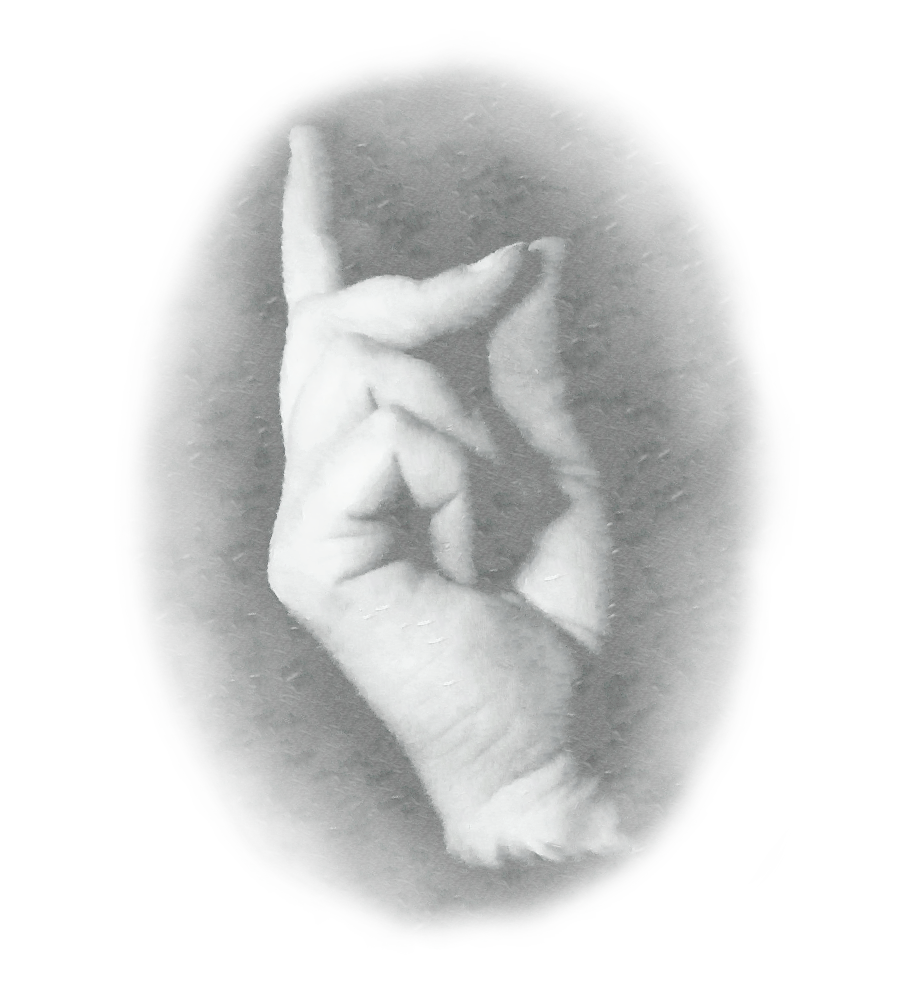
\includegraphics[scale=0.5]{bubble0.png} 

\vspace*{0.5cm}
\LARGE\lumos{Eliezer {\kern 1ex}Yudkowsky}
\normalsize

\vspace{2.0cm}
Find the original text at:\\
\url{http://hpmor.com} \\
{\scriptsize \url{http://www.fanfiction.net/s/5782108}} \\

\end{center}
\end{vplace}

% Credit to Rowling on verso page
\cleartoverso

\begin{center}
\vspace*{2.0cm}

\thispagestyle{empty}
Based on the characters of

\vspace*{0.5cm}

\Large J. K. ROWLING \normalsize 

\vspace*{0.5cm}

and her books:

\vspace*{0.5cm}

{
	\newcounter{books_list_counter}
	\def \hpBook #1{  
		\addtocounter{books_list_counter}{1} 
		\textit{Harry Potter and the #1} \par
		Year \numtoName{\value{books_list_counter}} at Hogwarts
		\smallskip\par
	}
	
	\hpBook{Sorcerer’s Stone}
	\hpBook{Chamber of Secrets}
	\hpBook{Prisoner of Azkaban}
	\hpBook{Goblet of Fire}
	\hpBook{Order of the Phoenix}
	\hpBook{Half-Blood Prince}
	\hpBook{Deathly Hallows}
}
\end{center}


% Begin subbook title

\cleartorecto

\begin{vplace}
\begin{center}
\thispagestyle{empty}

\HUGE{\hp book \hpBookNo} \vspace*{1.0cm}

\normalsize\lumos{\hpBookChar} \vspace*{0.2cm}

\footnotesize\lumos{and the}

\large\lumos{\hpBookTitle} \vspace*{0.5 cm}

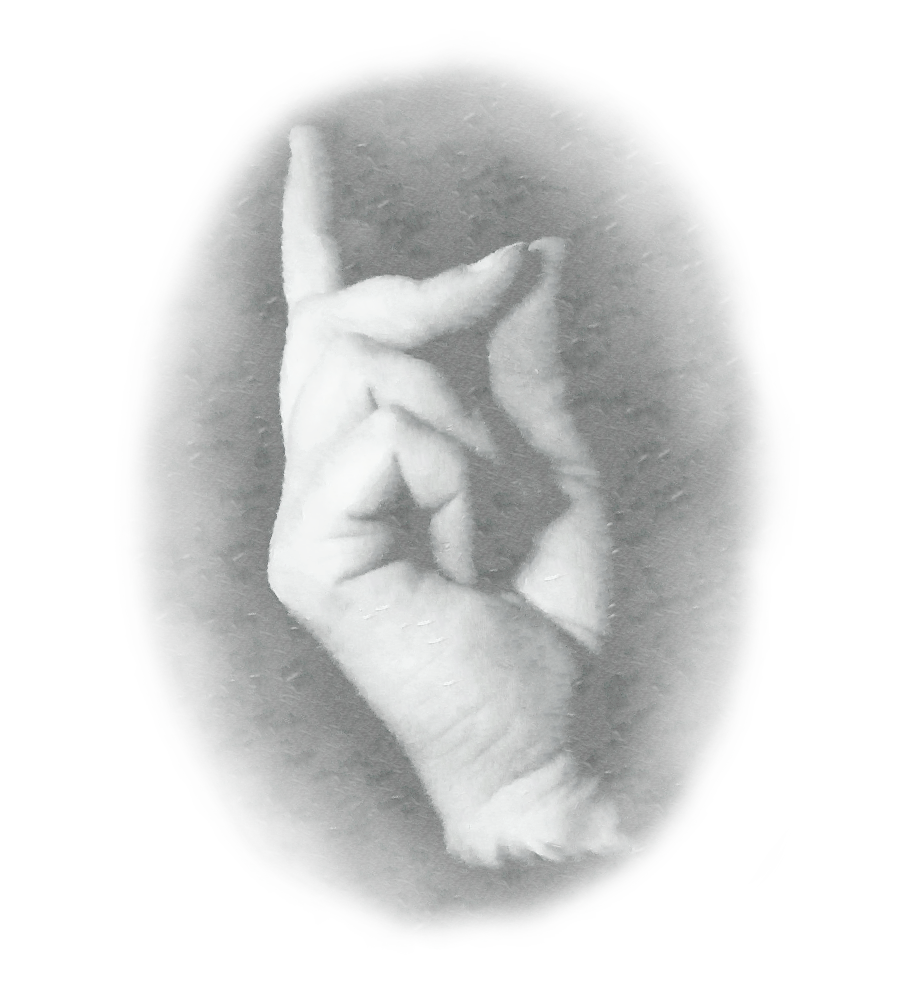
\includegraphics[scale=0.4]{bubble0.png} 

\vspace*{0.5cm}
\LARGE\lumos{Eliezer {\kern 1ex}Yudkowsky}

\vspace*{1.5cm}
\Large \hpBookChapters

\vspace*{0.5cm}
\scriptsize \hpBookOther \normalsize

\end{center}
\end{vplace}

% End subbook title
